\subsubsection{Data Path} \label{fpga:fitness:sss:data_path}
The design of the fitness core is highly influenced by the classic pipelined MIPS core design\cn.
The core is designed as a five stage pipeline.
The contents of the different stages in the pipeline, however, differs from the original MIPS architecture, as the CPU architecture has to accomadate for the ISA design which combines ideas from multiple exisiting architectures.
An overview of the data path can be seen in figure \vref{fpga:fig:fitness:fitness_arch}

\begin{figure}

  \centering
  % Trim er [left bottom right top]
  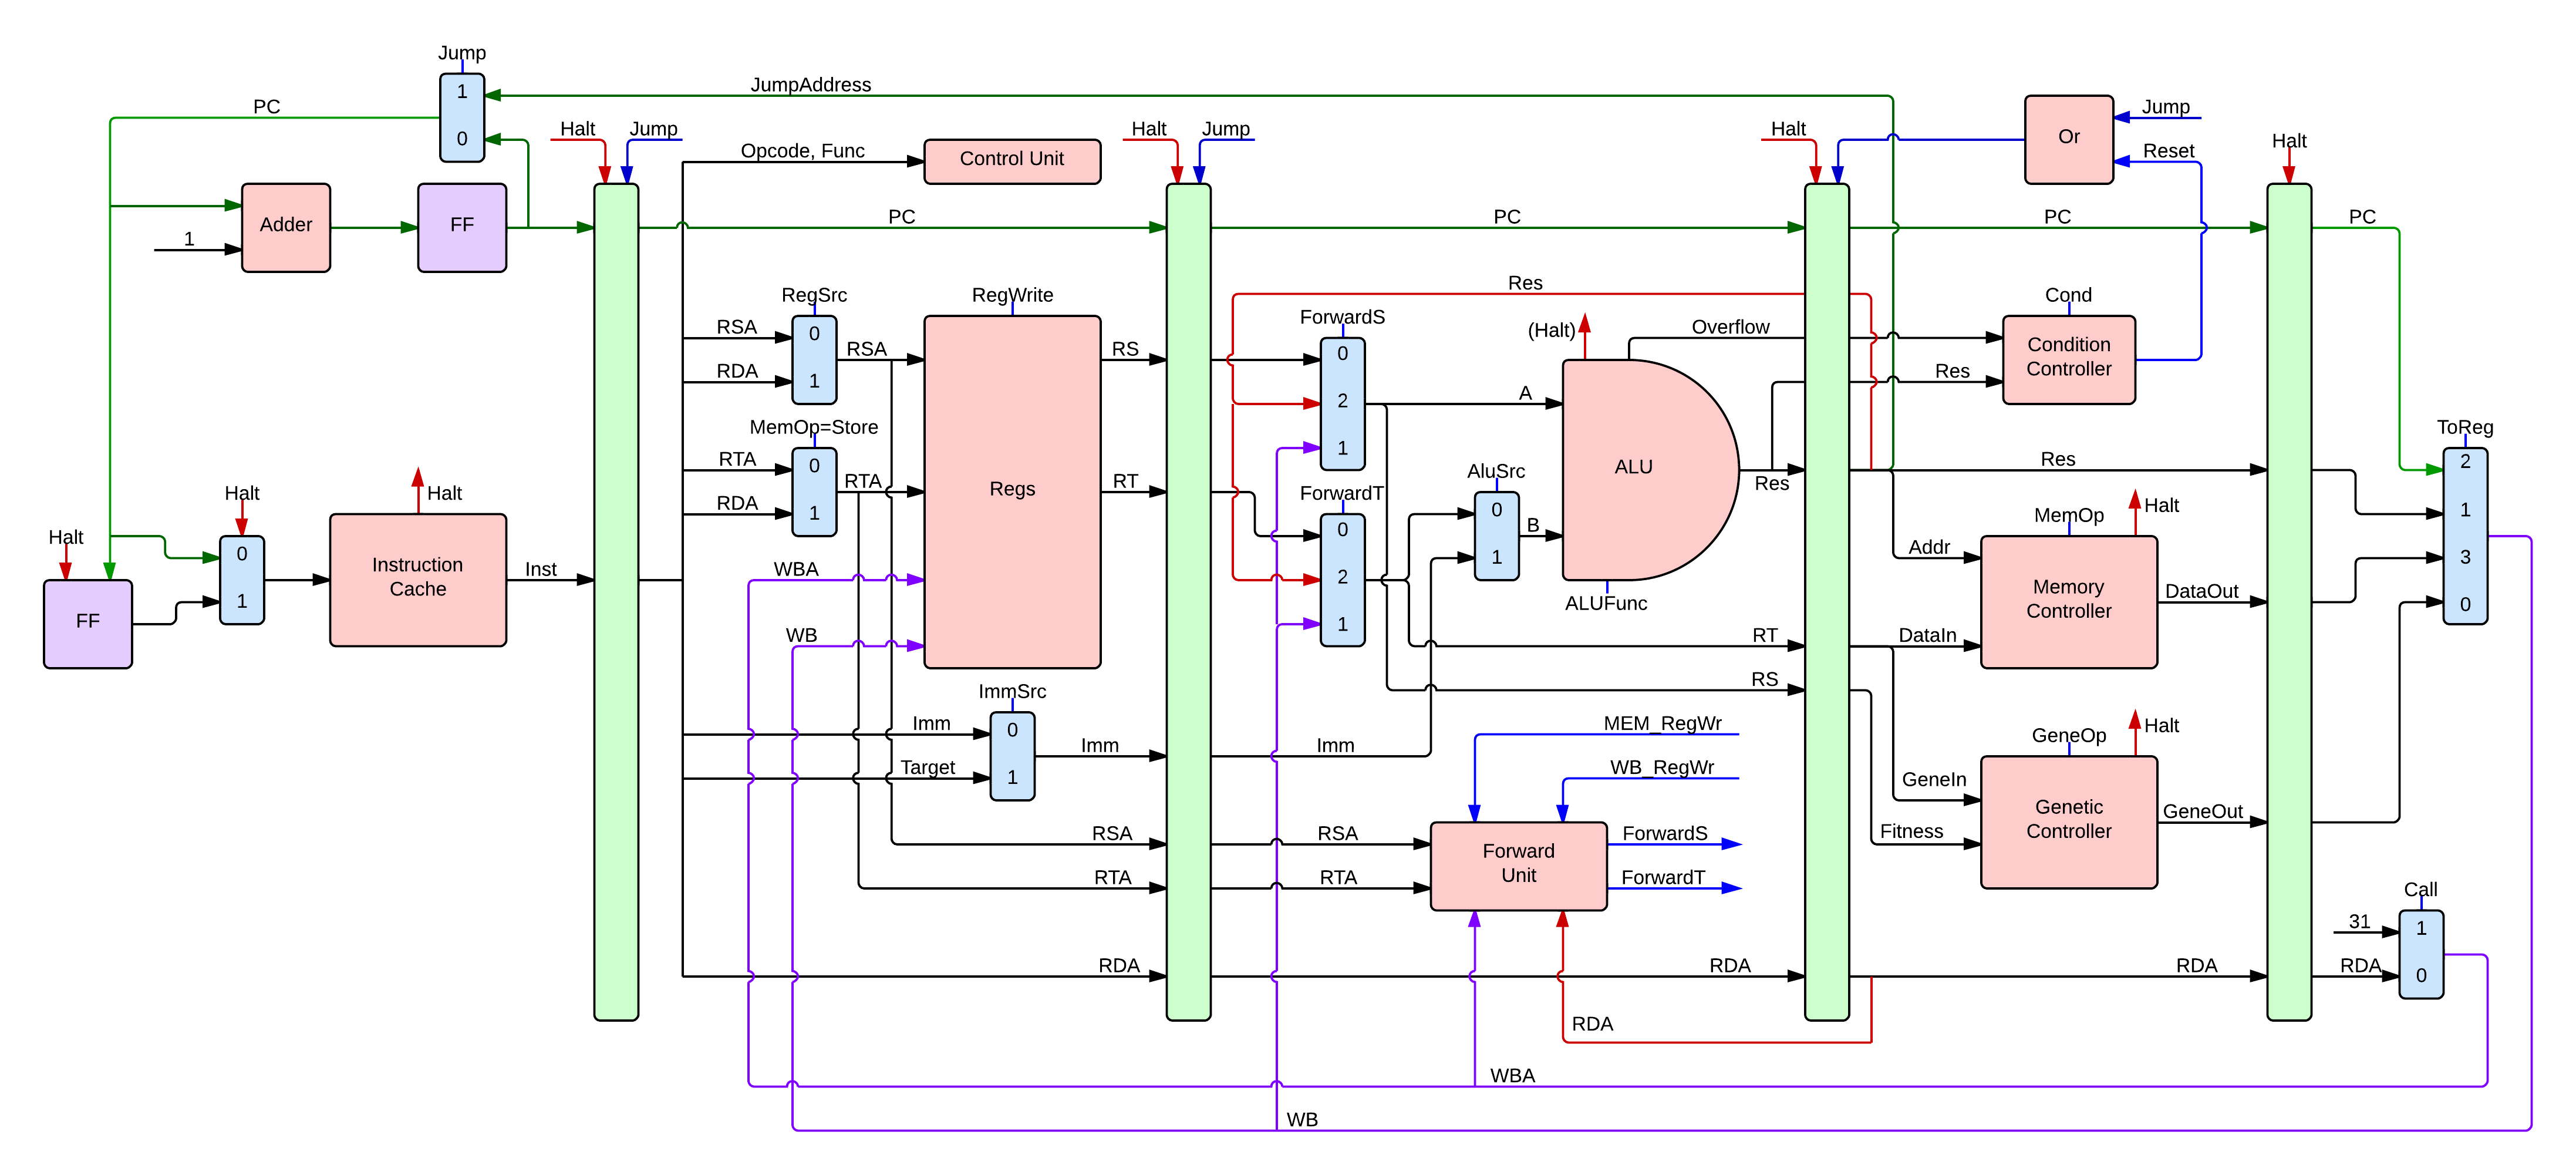
\includegraphics[width=\textwidth]{fpga/fig/fitness_core.png}
  \caption{Architecture block diagram}
  \label{fpga:fig:fitness:fitness_arch}
\end{figure}
.

The data path is simple.
The instruction is the same length for all the instructions.
This makes it easier to fetch the instruction in the first stage and decode it in the second.
Also, the ISA only supports three different instructions classes with the register mappings located on the same positions.
This allows the register file to be read on the same time as the control unit determines the correct control signals for that particular instruction.
This allows for a shorter pipeline.
If the instruction format where not symmetric, we would need to split the register file and decode stage in two stages.
A bigger pipeline would imply higher risk for pipeline hazards, and a more complicated hazard detection and correction schemes. 

The data path is in fact a load/store architecture.
This simplifies the execution and memory interaction.
Note that memory operands only appear in load and store instructions.
This implies that the execution stages is responsible for calculating the memory address and that the memory access can happen in the following stage.
Allowing the ALU to operate on operands in memory would expand the address stage, memory stage and the execution stage \cite[p.~335]{compOrgDes}.
The resulting architecture would involve a deeper pipeline. 



The MIPS inspired pipeline allows the design to be simple, but still powerful.
It  will increase performance by effectively increasing the instruction throughput.
Note that instruction throughput is an important metric because real applications execute millions of instructions \cite[p.~335]{compOrgDes}



More advanced features like branch prediction and instruction scheduling are not taken into consideration while designing the data path.
The group decided that the overall design should be as simple as possible.
Hazard and branching schemes are kept simple.
Hazards are resolved with the \emph{forwarding unit}, which forwards data if dependencies are detected.
Branching are resolved with use of \emph{conditional} codes in each instructions.
The reader may refer to their respective sections for more details.



\subsubsection{Control Unit} \label{fpga:fitness:sss:control_unit}
In order to execute different instructions classes in the data path there is need for a control unit.
The responsibility of the control unit is to configure all the different components for the current CPU operation so that the desired computation will emerge from the flow of data.
The control unit achieves this by setting the control signals of the relevant control signals of the relevant components to the values associated with the current instruction.
Note that different instructions classes requires different use of the data path.
Thus, combinations the control signals must accommodate the different instructions formats.



The control unit sets up the components based on the \emph{FUNCTION CODE} and the \emph{OPERATION CODE} of the instruction.


\input{fpga/tbl/fitness_core_control_unit_tbl}

    



\subsubsection{Conditionals} \label{fpga:fitness:sss:conditionals}
Like ARM , the galapagos architecture use conditional codes in order to determine if an instruction should be executed or not.
Instead of using explicit branch instructions every instruction carries a 4-bit conditional code.
Every instruction is in fact executed, however, the effect of the instruction is determined by the \emph{condition unit}.



\subsubsection{The ALU}\label{fpga:fitness:sss:the_alu}

\subsubsection{Forwarding Unit} \label{fpga:fitness:sss:forwarding_unit}
Since the executions of instructions overlap in the pipeline.
There is need for some mechanism to handle the data dependencies that arise between the instructions.
These data dependencies are known as data hazards.
They occur when a planned execution of an instruction is not possible because the data required is not yet available in the register file.
This particular problem can be solved in two ways, either by stalling or by forwarding.
Stalling, the simplest solution, is done by simply avoid these hazards by inserting \emph{NOPs} in the pipeline.
This solution works well, but are to slow for most cases.
Since this processors aim to achieve high performance this solution is far from optional.
A far better approach is to rely on forwarding, also known as register forwarding.
In this approach the aim is to resolve the dependencies by simply forwarding values from other stages if needed.
This will work in most cases, since even though the value does not yet reside in the register file, the value reside deeper in the pipeline.






\subsubsection{Memory Controller} \label{fpga:fitness:sss:memory_controller}

\subsubsection{Genetic Pool Controller} \label{fpga:fitness:sss:genetic_pool_controller}

\subsubsection{Case Study} \label{fpga:fitness:sss:case_study}




\fxnote {The hazard scheme may change if time}
